\chapter{What Counts as Capital}

At this point in the road, many people feel that the subject has finally arrived: money.

That feeling is understandable, but it is also a warning. Wealth freedom is not built by talking about money alone. If money were the whole subject, the earlier chapters on attention, payment, safety, the future, and benefactors would have been unnecessary. Yet those chapters are not decoration. They are preparation.

A person who cannot govern attention cannot use capital well. A person who cannot pay for progress will avoid the very tools that increase future earning power. A person ruled by safety will never give time enough room to work. A person who cannot live partly in the future will be shaken by every short-term movement. A person who cannot build trust will be cut off from many forms of opportunity.

So when we finally speak about capital, we are not leaving those ideas behind. We are discovering why they mattered.

\section*{Money Is Not Yet Capital}

A house is made mainly of bricks. But a pile of bricks is not a house.

Capital is made mainly of money. But a pile of money is not capital.

This distinction is simple, but many people never make it. They treat ``having money'' and ``having capital'' as the same thing. They are not the same. Money is a raw material. Capital is money arranged under conditions that allow it to produce more value.

A stack of bricks becomes a house only when design, time, labor, structure, and purpose are added. A sum of money becomes capital only when it is large enough for the chosen use, can be used long enough, and is guided by judgment.

\begin{center}
\begin{adjustbox}{max width=\linewidth}
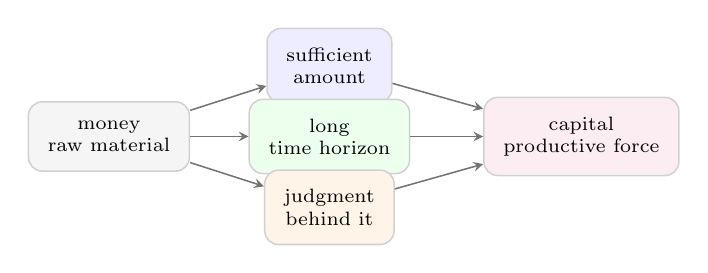
\begin{tikzpicture}[font=\scriptsize, line width=0.55pt, >=stealth]
  \node[draw=black!18, fill=gray!8, rounded corners=5pt, align=center, inner sep=7pt] (money) at (0,0) {money\\raw material};
  \node[draw=black!18, fill=blue!7, rounded corners=5pt, align=center, inner sep=7pt] (amount) at (2.8,0.9) {sufficient\\amount};
  \node[draw=black!18, fill=green!7, rounded corners=5pt, align=center, inner sep=7pt] (time) at (2.8,0) {long\\time horizon};
  \node[draw=black!18, fill=orange!9, rounded corners=5pt, align=center, inner sep=7pt] (wisdom) at (2.8,-0.9) {judgment\\behind it};
  \node[draw=black!18, fill=purple!7, rounded corners=5pt, align=center, inner sep=7pt] (capital) at (6.0,0) {capital\\productive force};
  \draw[->, draw=black!55] (money) -- (amount);
  \draw[->, draw=black!55] (money) -- (time);
  \draw[->, draw=black!55] (money) -- (wisdom);
  \draw[->, draw=black!55] (amount) -- (capital);
  \draw[->, draw=black!55] (time) -- (capital);
  \draw[->, draw=black!55] (wisdom) -- (capital);
\end{tikzpicture}
\end{adjustbox}
\end{center}

At least three elements are required.

\begin{enumerate}
\item The amount of money.
\item The length of time for which the money can be used.
\item The wisdom behind the money.
\end{enumerate}

The first element is obvious enough. One hundred yuan cannot be treated as capital in most meaningful investment settings. One million may be capital or may not be, depending on the field. Ten billion seems large enough in almost every field, yet even ten billion is not automatically capital if it is not under the right conditions.

The second element is more important than most people imagine. How long can the money remain in use? One day, one month, one year, ten years, or forever are radically different conditions. The same amount of money has different power depending on its usable time.

Money that must be withdrawn soon is not the same as money that can wait. Money that may be needed for rent next month cannot behave like money that can sit for a decade. Money that shakes your sleep is not the same as money that can endure market weather without pulling your mind apart.

The third element is the most important: the wisdom behind the money. The same sum in different hands has different force. Give the same starting amount to a beginner, a careful operator, and a first-rate investor, and the results will not merely differ by luck. They will differ because of judgment, preparation, networks, patience, selection, and the ability to see what others cannot yet see.

This is a hard sentence, but it is useful:

\begin{quote}
Most people are not yet qualified to stand behind capital.
\end{quote}

That sentence is not an insult. It is a diagnostic. It tells us what must be built.

\section*{The Time Element}

Consider a well-known example from Chinese business history. In 1988, Liu Yuansheng bought 3.6 million shares of Vanke for 3.6 million yuan. For decades, he did not sell. By June 27, 2016, when Vanke's market capitalization was about 269.7 billion yuan, his position was worth roughly 2.7 billion yuan. That is about 750 times in 28 years.

The impressive number is not only the return. The deeper fact is that the original money could remain untouched for so long. For him, that money did not need to be rescued for daily life, emergency repair, social display, or emotional comfort. It could be sentenced to time.

Most people who put money into the stock market do not have this condition. Their money is noisy. It is tied to rent, marriage, pride, anxiety, debt, comparison, or next year's plan. Once the price moves, the person moves with it. Their mood rises and falls with the chart. Their attention, which is their most precious asset, is consumed by price movement.

Even if such a person earns money, the trade may still be bad if it destroys attention. If they lose money too, then both money and attention have been sacrificed.

This is why not every market participant is an investor. Many are only nervous owners of money inside an investment-looking environment.

\section*{Relative Returns Matter More Than Absolute Amounts}

The first breakthrough is usually not increasing the amount of money. The first breakthrough is changing the measurement.

Many people refuse to begin because they say, ``I do not have much money anyway.'' This sounds practical, but it is often self-protection. If investment is only for people with large sums, then the person with a small sum can avoid learning. They can even despise the learners and call them petty, calculating, or foolish.

The real issue is not the absolute amount of profit or loss. The real issue is the ratio.

If one person invests 10,000 yuan and earns 50\%, while another invests 100,000 yuan and earns 15\%, the second person earns more money in absolute terms, but the first person has used capital more efficiently. In percentage terms, the first result is better.

This is elementary mathematics, yet many adults do not apply it to life. They look at prices and amounts, not ratios. They avoid a good asset because it ``looks expensive'' and chase a poor asset because it ``looks cheap.'' They confuse the number printed on the price tag with the quality of the opportunity.

The compound formula makes the issue plain:

\[
(1+r)^n
\]

The variable \(r\) is the rate of return. The variable \(n\) is the number of periods. A small beginning is not a reason to refuse growth. Everyone starts from their own base. What matters is whether the base compounds.

Comparison ruins many people here. They look at someone else's starting point and conclude that their own step is too small to matter. But a step is measured first against your own starting point. If it increases your capacity, it matters.

The relative view removes many unnecessary burdens. It allows a person with modest means to begin practicing seriously. It also prevents a person with larger means from feeling proud of poor efficiency.

\section*{Sentence Some Money to Life}

The most important breakthrough is this:

\begin{quote}
Can you sentence part of your investment money to life imprisonment?
\end{quote}

The phrase is deliberately severe. It means money that you can treat as unavailable for ordinary life. Money that does not need to be pulled back for consumption, emergency vanity, fear, or convenience. Money that can remain in the field long enough for judgment, learning, and compounding to develop.

For many people, this sounds impossible only because they have not examined the real numbers.

Suppose a person earns 60,000 yuan a year. Setting aside 5,000 yuan as long-term investment money may not actually reduce life quality in any serious way. Psychological research often finds that many people could lose a modest percentage of annual income without a corresponding collapse in daily life quality. The pain is often larger in imagination than in reality.

This does not mean everyone should act carelessly. It means people should stop lying to themselves. The question is not, ``How much would I enjoy losing?'' No one enjoys loss. The question is, ``What amount could I truly leave alone without damaging my life?''

For one person it may be 5,000 yuan. For another, 50,000. For another, much less. The number itself is not sacred. The honesty is sacred.

Money that cannot be calmly sentenced to a long term should not pretend to be capital. If the money will soon be needed, it is not capital. If losing it would destroy your basic life, it is not capital. If every movement will hijack your attention, it is not capital. It is only anxious money wearing an investor's clothes.

This connects to the earlier chapter on safety. The goal of wealth freedom is not to become reckless. One of the secrets of gaining wealth is to avoid unnecessary risk. Abandoning false safety does not mean worshiping danger. It means freeing enough attention to study, observe, and act over a long horizon.

\section*{Wisdom Comes Through Practice}

The third breakthrough, wisdom, is joined to the second.

Investment wisdom cannot be gained only by reading books, listening to experts, or repeating famous sentences. Those things may help, but they are not yet yours. Knowledge becomes yours only after it enters action, meets consequences, survives correction, and grows roots.

This process cannot be skipped by intelligence. Some things simply require time. A child cannot be born healthy after five months because the parents are clever. In the same way, investment judgment cannot become mature without repeated contact with reality.

This is another reason the investment amount should begin within a range that permits calm. If the amount is too large relative to your life, you will not learn well. You will panic, defend, rationalize, imitate, or gamble. You will not observe clearly.

The loop should look more like this:

\begin{center}
\begin{adjustbox}{max width=\linewidth}
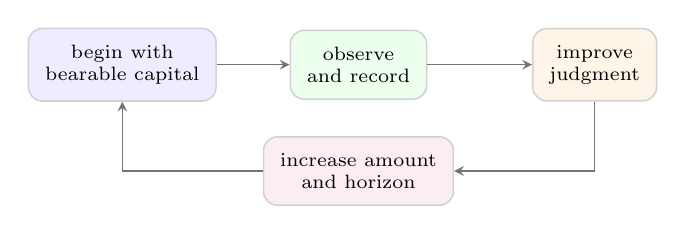
\begin{tikzpicture}[font=\scriptsize, line width=0.55pt, >=stealth]
  \node[draw=black!18, fill=blue!7, rounded corners=5pt, align=center, inner sep=6pt] (small) at (0,0) {begin with\\bearable capital};
  \node[draw=black!18, fill=green!7, rounded corners=5pt, align=center, inner sep=6pt] (observe) at (3.0,0) {observe\\and record};
  \node[draw=black!18, fill=orange!9, rounded corners=5pt, align=center, inner sep=6pt] (judge) at (6.0,0) {improve\\judgment};
  \node[draw=black!18, fill=purple!7, rounded corners=5pt, align=center, inner sep=6pt] (larger) at (3.0,-1.35) {increase amount\\and horizon};
  \draw[->, draw=black!55] (small) -- (observe);
  \draw[->, draw=black!55] (observe) -- (judge);
  \draw[->, draw=black!55] (judge) |- (larger);
  \draw[->, draw=black!55] (larger) -| (small);
\end{tikzpicture}
\end{adjustbox}
\end{center}

Amount, time horizon, and wisdom improve together. The mistake is waiting for a large amount before beginning. Without practice, the large amount may only magnify ignorance.

This is why relying on experts is often a weak form of investment. Good investing is finally a ``no one can replace me'' activity. Other people can inform you, challenge you, teach you, and warn you. They cannot lend you their judgment in a form that removes your responsibility.

A person without their own investment concepts usually explains decisions with borrowed phrases: a friend recommended it, an expert said so, there is inside information, everyone is buying, it looks cheap, it cannot fall much more. These are not reasons. They are ways of hiding the absence of reasons.

\section*{Investment and Gambling}

The surface of investing and gambling can look similar. Money is placed. The future is uncertain. Results fluctuate.

The difference lies underneath.

Investment requires investigation, judgment, a time horizon, risk control, and a reasoned expectation that value will grow. Gambling depends on excitement, leverage, rumor, urgency, and the hope that uncertainty will be kind.

Some gamblers win. That proves almost nothing. If you envy the person who used leverage and became rich, you should also study the many people who used leverage and disappeared. They are part of the same category. One is the lucky visible edge. The other is the buried cost.

Borrowing money to invest is dangerous in most ordinary cases because it damages all three elements of capital.

\begin{enumerate}
\item The amount is not truly positive; it begins under the weight of debt.
\item The time horizon is usually short, because debt has pressure and deadlines.
\item The very choice often shows insufficient wisdom about the first two points.
\end{enumerate}

Borrowing to gamble is worse. It joins negative capital to negative judgment.

The disciplined investor is not trying to feel brave. The disciplined investor is trying to survive long enough for correct judgment to compound.

\section*{Can, But May Choose Not To}

There is a subtle distinction that changes the way the mind works:

\begin{quote}
Wanting something but being unable to do it is different from being able to do it but choosing not to.
\end{quote}

A person who never received an admission letter and says, ``I did not want to go to that university anyway,'' is not in the same position as a person who received the letter and then chose a different path. The outward sentence may sound similar. The inner structure is completely different.

The same is true with capital. A person who cannot sentence money to a long term but later happens not to touch it for two years is not in the same position as a person who could sentence it to a long term and then deliberately chose to end the period after two years. The result may look the same. The agency is different.

Agency matters. It changes attention, posture, patience, and learning.

This is visible in many areas of life. Two people may both be in graduate school. One returned because their knowledge was insufficient for the work they wanted to do. The other stayed because they could not find a job and needed to hide from the market for two more years. The outward label is the same. The inner condition is not.

People who become exceptional often share this trait: they actively choose. They are not merely pushed by fear, trend, debt, envy, or lack of options. They create options, then decide.

Capital requires this same posture. The money must not be driven by panic. It must be placed by choice.

\section*{Doing the Right Thing}

A sentence from the previous chapter returns with more force here:

\begin{quote}
Doing the right thing is more important than doing things right.
\end{quote}

If the money is not truly capital, clever tactics cannot save it. If the time horizon is wrong, better chart-reading may only create more frequent anxiety. If the person behind the money lacks judgment, more information may only produce more confident mistakes.

The right thing is to build the conditions under which money can become capital.

That means spending less attention on the fantasy of sudden profit and more attention on the three elements:

\begin{center}
\begin{tabular}{p{0.27\linewidth}p{0.62\linewidth}}
\hline
Element & Practical question \\
\hline
Amount & What sum can I set aside without damaging ordinary life? \\
Time & Can this sum remain untouched long enough to learn and compound? \\
Wisdom & What do I understand well enough to judge for myself? \\
\hline
\end{tabular}
\end{center}

This table is small, but it can expose a large lie. Many people say they are investing when they have no clear answer to any of the three questions.

\section*{The Five-Thousand-Yuan Test}

Use a simple number as a mirror: 5,000 yuan.

Do not treat it as a universal rule. Treat it as a thinking tool.

If serious investment practice could begin with 5,000 yuan, when could you first have begun? How many years have passed since then? How much time did you miss? That time was not abstract. It was part of your limited life.

If serious investment practice could begin with 5,000 yuan, how many people around you already have the means to begin, yet have never realized that they can? How much longer will they wait because they believe the first step must be large?

Now replace 5,000 with your own real number. What amount can you truly sentence to a long term? If the answer is ``not enough,'' what number do you believe is enough? How long will it take to prepare that number? What must change in your spending, earning, attention, or self-image for that number to become real?

If you have already begun investing, ask a harsher question: does the money you use deserve to be called capital? Can it wait? Can you wait? Is there judgment behind it? Or is it only restless money seeking excitement, comparison, or rescue?

These questions are uncomfortable because they remove excuses. But discomfort is useful when it points to structure.

\section*{Capital Begins Before Wealth}

The good news is that the threshold is lower than most people imagine after the concept is corrected. The bad news is that the threshold remains invisible to anyone who refuses the concept.

For a person with outdated ideas, the road is full of chasms: not enough money, not enough luck, not enough connections, not enough timing, not enough expert advice. For a person who understands capital, the first steps become concrete: define a bearable amount, lengthen the time horizon, practice judgment, protect attention, and repeat.

This does not guarantee exceptional investment results. Nothing honest can guarantee that. But it creates the basic condition without which results are mostly illusion.

The thought about capital should not stop after this chapter. In coming chapters, we will return to ideas that appear unrelated to wealth: backwardness, multidimensional competition, metacognition, persistence, correctness, self-drive, and execution. Those ideas will again seem distant from money. They are not distant.

Capital is not merely money. Capital is money plus time, judgment, attention, and the person's whole operating system behind it.

If the person is not ready, money remains money. It may even become someone else's capital. If the person becomes ready, even a modest amount can begin the long education.

That is where wealth freedom becomes less mysterious. It does not begin when a large pile of money appears. It begins when a person becomes capable of turning money into capital.
